\section{Date: 2024-09-28}
\noindent \textbf{Series ID: PECILBU18MA25023A647NCEN} 

\noindent This series is titled 90% Confidence Interval Lower Bound of Estimate of People Age 0-17 in Poverty for Plymouth County, MA and has a frequency of Annual. The units are Persons and the seasonal adjustment is Not Seasonally Adjusted.The observation start date is 1989-01-01 and the observation end date is 2022-01-01.The popularity of this series is 1. \\ 

\noindent \textbf{Series ID: DLTRUCKSNSA} 

\noindent This series is titled Motor Vehicle Retail Sales: Domestic Light Weight Trucks and has a frequency of Monthly. The units are Thousands of Units and the seasonal adjustment is Not Seasonally Adjusted.The observation start date is 1967-01-01 and the observation end date is 2024-08-01.The popularity of this series is 4. \\ 

\subsection{\subsection{Regression Tables and Plots}}
\begin{center}
\begin{tabular}{lclc}
\toprule
\textbf{Dep. Variable:}                        & value\_fred\_DLTRUCKSNSA & \textbf{  R-squared:         } &     0.354   \\
\textbf{Model:}                                &           OLS            & \textbf{  Adj. R-squared:    } &     0.330   \\
\textbf{Method:}                               &      Least Squares       & \textbf{  F-statistic:       } &     14.80   \\
\textbf{Date:}                                 &     Sat, 28 Sep 2024     & \textbf{  Prob (F-statistic):} &  0.000663   \\
\textbf{Time:}                                 &         16:52:48         & \textbf{  Log-Likelihood:    } &   -169.80   \\
\textbf{No. Observations:}                     &              29          & \textbf{  AIC:               } &     343.6   \\
\textbf{Df Residuals:}                         &              27          & \textbf{  BIC:               } &     346.3   \\
\textbf{Df Model:}                             &               1          & \textbf{                     } &             \\
\textbf{Covariance Type:}                      &        nonrobust         & \textbf{                     } &             \\
\bottomrule
\end{tabular}
\begin{tabular}{lcccccc}
                                               & \textbf{coef} & \textbf{std err} & \textbf{t} & \textbf{P$> |$t$|$} & \textbf{[0.025} & \textbf{0.975]}  \\
\midrule
\textbf{const}                                 &     752.4154  &       73.373     &    10.255  &         0.000        &      601.866    &      902.965     \\
\textbf{value\_fred\_PECILBU18MA25023A647NCEN} &      -0.0299  &        0.008     &    -3.847  &         0.001        &       -0.046    &       -0.014     \\
\bottomrule
\end{tabular}
\begin{tabular}{lclc}
\textbf{Omnibus:}       &  4.911 & \textbf{  Durbin-Watson:     } &    0.707  \\
\textbf{Prob(Omnibus):} &  0.086 & \textbf{  Jarque-Bera (JB):  } &    3.382  \\
\textbf{Skew:}          & -0.798 & \textbf{  Prob(JB):          } &    0.184  \\
\textbf{Kurtosis:}      &  3.502 & \textbf{  Cond. No.          } & 4.26e+04  \\
\bottomrule
\end{tabular}
%\caption{OLS Regression Results}
\end{center}

Notes: \newline
 [1] Standard Errors assume that the covariance matrix of the errors is correctly specified. \newline
 [2] The condition number is large, 4.26e+04. This might indicate that there are \newline
 strong multicollinearity or other numerical problems.

\begin{figure}
\centering
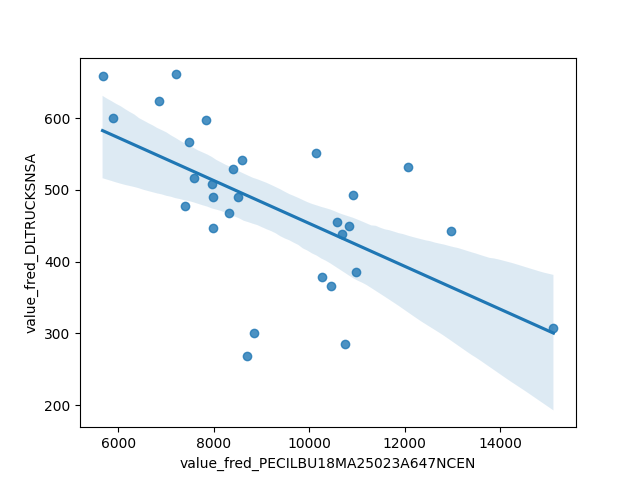
\includegraphics[scale = 0.9]{plots/plot_2024-09-28.png}
\caption{Regression Plot for 2024-09-28}
\end{figure}
\newpage
